\chapter{Eigenvalues for Infinite-Medium Problems}% for the Rayleigh Quotient Fixed Point Method}

In this chapter we describe the performance of the Rayleigh quotient methods for various infinite-medium problem selected from the \textit{Analytical Benchmark Test Set for Criticality Code Verification} \cite{sood2003analytical} or analytical benchmark solutions. Some problems were selected that did not meet the assumptions used in deriving the RQFP methods to test the general applicability of the methods. For example, problems with anisotropic scattering and fissioning only in specific energy groups were selected to verify whether the RQFP methods would converge when the primitivity condition no longer applied. The Rayleigh quotient method was compared to the critical search method \cite{hill_efficient_1983} for alpha-eigenvalue problems and to standard power iteration for $k$-effective eigenvalue problems. The total number of transport sweeps, the action of $\mathbf{H}_{\mathbf{z}}^{-1}$ on the source vector, was compared for each method as they represent the majority of computational expense in standard transport codes. The methods were implemented in ARDRA, a 1D, 2D, and 3D deterministic discrete ordinates neutron and gamma transport code developed and maintained by Lawrence Livermore National Laboratory \cite{hanebutte_ardra_1999}.

\section{Criticality Benchmark One-Speed Verification for Various Critical and Supercritical Problems}

A set of six one-material infinite-medium supercritical problems were selected from the \textit{Analytical Benchmark Test Set for Criticality Code Verification} \cite{sood2003analytical} to test the Rayleigh Quotient Fixed Point method for both alpha-eigenvalue and $k$-effective eigenvalue problems. Each problem was modeled as a slab with reflective boundary conditions on both sides. The slab was discretized using diamond differencing discretization in space ($M = 2$) and S$_{2}$ discrete ordinates Legendre quadrature ($L = 2$) in angle \cite{lewis_computational_1984}. The eigenvector/eigenvalue residual was converged to a tolerance of $10^{-12}$. These problems were selected as they contained cross sections of commonly used fissile isotopes in nuclear engineering applications such as plutonium-239 and uranium-235 (Table~\ref{table:SoodInf}). Sood Criticality Benchmark Problems 1 and 5 consisted of two sets of plutonium-239-like cross sections, each with a different $k_{\infty}$ values. Sood Criticality Benchmark Problems 11, 15, 17, and 19 consisted of four uranium-235-like cross section sets used to characterize a system approaching the critical state. The reference eigenvalues for these problems can be seen in Table~\ref{table:InfMed}. For one-speed problems, the velocity was set to $1$ cm/s unless otherwise noted.

\begin{table}[!t]
	\caption{Sood Criticality Benchmark Infinite-Medium Problem Cross Sections (cm$^{-1}$) in \cite{sood2003analytical}}
	\label{table:SoodInf}
	\begin{subtable}[h]{1.0\textwidth}
	\centering\ra{1.3}
    \begin{tabular}{*5c}
        \toprule
	Cross Section Set & $\sigma$ & $\nu \sigma_{f}$ & $\sigma_{s}$  & $v$ [cm/s] \\ 
        \midrule
	Sood Prob. 1 & 0.32640 & 0.264384 & 0.225216 & 1.0 \\
	Sood Prob. 5 & 0.231744 & 0.264384 & 0.225216 & 1.0 \\
        \bottomrule
    \end{tabular}%
	\caption{Plutonum-239-like Cross Section Sets}
	\label{table:PU}
	\end{subtable}%
	\vspace{0.25cm}
	\begin{subtable}[h]{1.0\textwidth}
	\centering\ra{1.3}
    \begin{tabular}{*5c}
        \toprule
	Cross Section Set & $\sigma$ & $\nu \sigma_{f}$ & $\sigma_{s}$  & $v$ [cm/s] \\ 
        \midrule
	Sood Prob. 11 & 0.32640 & 0.176256 & 0.248064 & 1.0 \\
	Sood Prob. 15 & 0.32640 & 0.18259475328 & 0.248064 & 1.0 \\
	Sood Prob. 17 & 0.32640 & 0.17673306624 & 0.248064 & 1.0 \\
	Sood Prob. 19 & 0.32640 & 0.17489804544 & 0.248064 & 1.0 \\
        \bottomrule
    \end{tabular}%
	\caption{Uranium-235-like Cross Section Sets}
	\label{table:U}
	\end{subtable}
\end{table}

For the supercritical one-speed criticality benchmark problems, the alpha-eigenvalue Rayleigh Quotient Fixed Point method performed substantially better than the critical search method, reducing the number of transport sweeps by a factor of 30 (Table~\ref{table:CompInfSweeps}). Reductions in transport sweeps were achieved by removing the need for intermediate $k$-effective eigenvalue calculations. In the critical search method, two sets of $k$-effective eigenvalue calculations are required before the linear interpolation or extrapolation of the alpha-eigenvalue can be done. Subsequent updates of the alpha-eigenvalue are dependent on the bracketing procedure finding the correct alpha-eigenvalue. With each update of the alpha-eigenvalue requiring a converged $k$-effective eigenvalue calculation, the number of transport sweeps increases rapidly. The computation expense of one iteration of the alpha-eigenvalue RQFP method is the same as one iteration of the $k$-effective eigenvalue calculation. Since there is no need for any intermediate calculations, the Rayleigh Quotient Fixed Point method can calculate the eigenvalue/eigenvector pair directly, avoiding this drawback of the critical search method and drastically reducing the number of total sweeps necessary. In one particular instance, the bracketing procedure of the critical search method failed and the method did not converge. An example of the convergence behavior of the alpha-eigenvalue RQFP method is shown for the PUa cross section set infinite-medium problem in Figure~\ref{fig:AlphaInfConv}. These plots show that the convergence rate for the RQFP methods is linear in general for all problems. For these very supercritical systems, the Rayleigh Quotient Fixed Point method was able to calculate the supercritical alpha-eigenvalues without issue.

The RQFP for the $k$-effective eigenvalue reduces the number of sweeps by a factor of three (Table~\ref{table:CompInfSweepsK}) as compared to the power method with the fission source norm update. In these particular problems, all cells contain fissile material and the angular flux is exactly equal to the fission source to some constant. The rapid convergence of the angular flux by the Rayleigh Quotient Fixed Point method as compared to the power method with fission source norm update results in a substantial reduction in the number of transport sweeps necessary to converge the eigenvector/eigenvalue. While the convergence of the method is linear, it appears in practice to have a lower asymptotic constant coefficient than the power method as seen in Figure \ref{fig:kRes}.

\begin{table}[!htbp]
	\caption{Reference Eigenvalues and Transport Sweep Comparisons for Sood Criticality Benchmark Infinite-Medium Problems in \cite{sood2003analytical}}
	\label{table:InfMed}
	\begin{subtable}[h]{1.0\textwidth}
	\centering\ra{1.3}
	\begin{tabular}{@{}cccc@{}}\toprule
	& & \multicolumn{2}{c}{Transport Sweeps} \\
	\cmidrule{3-4} Cross Section Set & Reference $\alpha_{\infty}$ [s$^{-1}$] & RQFP & Critical Search\\
	\midrule
	Sood Prob. 1 & 0.1632 & 29 & 7,361 \\
	Sood Prob. 5 & 0.257856 & 40 & *   \\
	Sood Prob. 11& 0.09792 & 28 & 6,101 \\
	Sood Prob. 15 & 0.104258753 & 28 & 6,426 \\
	Sood Prob. 17 & 0.0983970662 & 28 & 6,114 \\
	Sood Prob. 19 & 0.0965620454 & 28 & 5,995 \\
	\bottomrule%
	\multicolumn{4}{l}{*Did Not Converge} \\
	\end{tabular}
	\caption{Alpha-Eigenvalue: Comparison of RQFP and Critical Search Transport Sweeps}
	\label{table:CompInfSweeps}
	\end{subtable}%
	\vspace{0.25cm}
	\begin{subtable}[h]{1.0\textwidth}
	\centering\ra{1.3}
	\begin{tabular}{@{}cccc@{}}\toprule
	& & \multicolumn{2}{c}{Transport Sweeps} \\
	\cmidrule{3-4} Cross Section Set & Reference $k_{\infty}$ & RQFP & Power Method \\
	\midrule
	Sood Prob. 1 & 2.612903 & 41 & 111 \\
	Sood Prob. 5 & 2.290323 & 34 & 96   \\
	Sood Prob. 11 & 2.25 & 29 & 130\\
	Sood Prob. 15 & 2.330917 & 30 & 132 \\
	Sood Prob. 17 & 2.256083 & 27 & 131 \\
	Sood Prob. 19 & 2.232667 & 33 & 131\\
	\bottomrule
%	\multicolumn{6}{l}{$M = 500$, $L = 64$, Tolerance = $10^{-12}$} \\
	\end{tabular}
	\caption{$k$-Effective: Comparison of RQFP and Power Method Transport Sweeps}
	\label{table:CompInfSweepsK}
	\end{subtable}
\end{table}

\begin{figure}[!htbp]
	\centering
	\noindent\begin{subfigure}[!htbp]{0.5\textheight}
		\centering
		\resizebox{1.0\textwidth}{!}{
		% This file was created by matlab2tikz.
%
%The latest updates can be retrieved from
%  http://www.mathworks.com/matlabcentral/fileexchange/22022-matlab2tikz-matlab2tikz
%where you can also make suggestions and rate matlab2tikz.
%
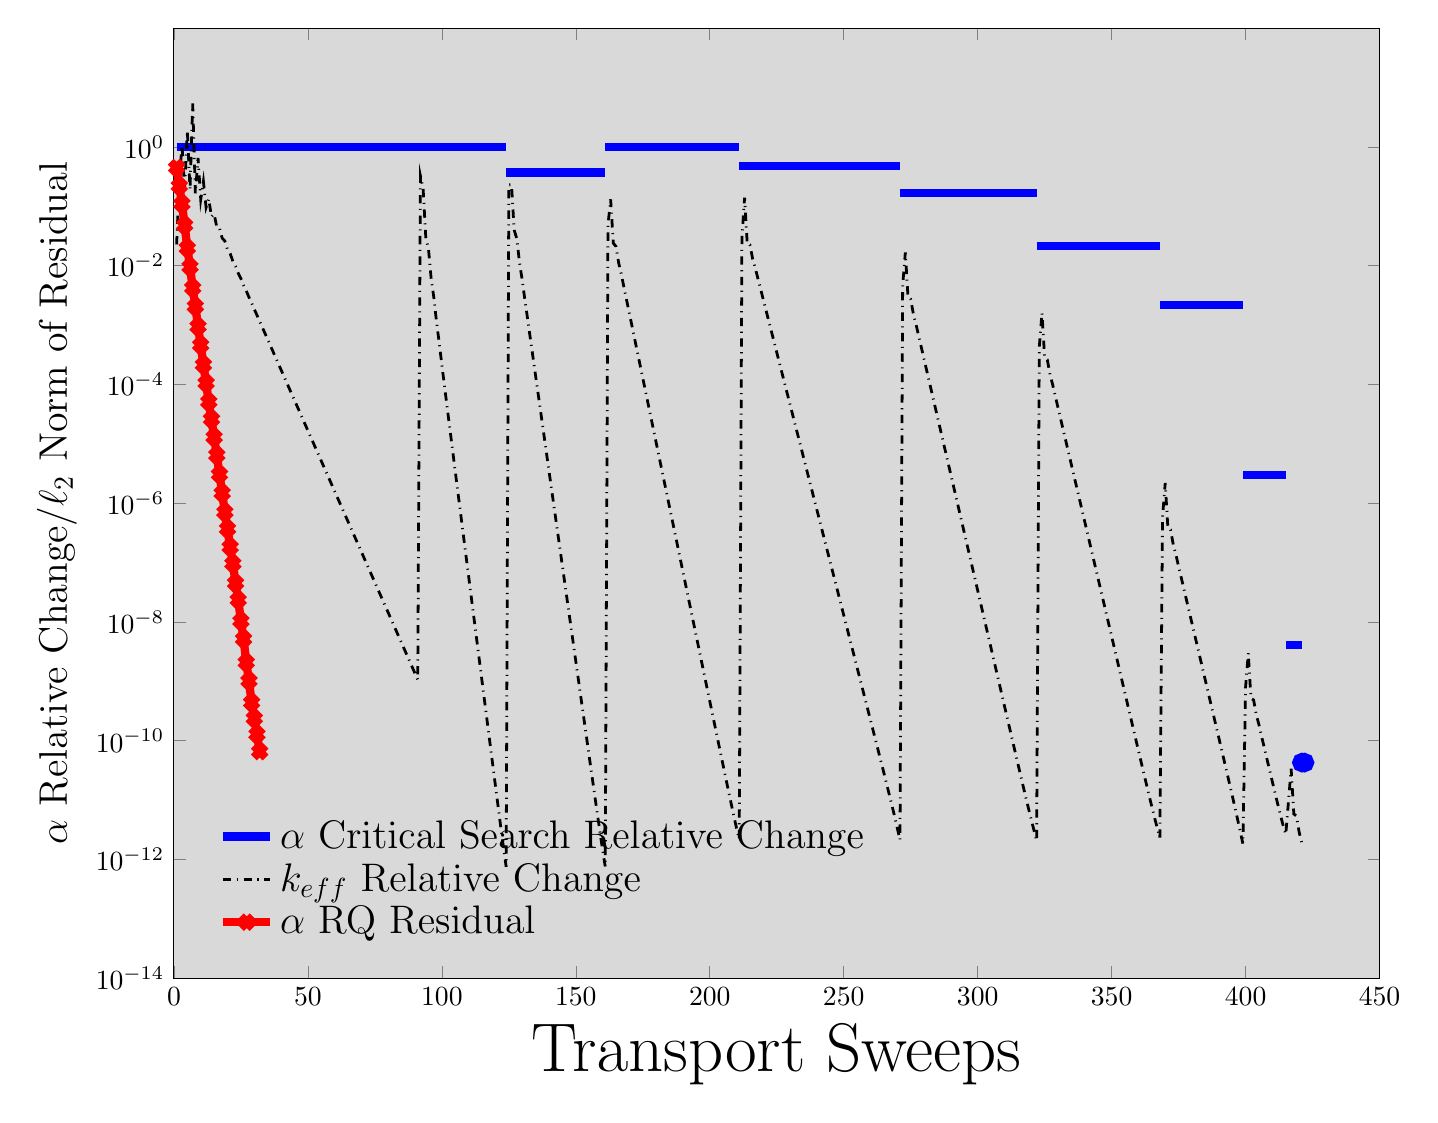
\begin{tikzpicture}

\begin{axis}[%
width=6.028in,
height=4.75in,
at={(1.011in,0.646in)},
scale only axis,
xmin=0,
xmax=450,
xlabel style={font=\color{white!15!black},font=\Huge},
xlabel={Transport Sweeps},
ymode=log,
ymin=1e-14,
ymax=100,
yminorticks=true,
ytick={1, 1e-2, 1e-4, 1e-6, 1e-8, 1e-10, 1e-12, 1e-14},
ylabel style={font=\color{white!15!black},font=\Large},
ylabel={$\alpha$ Relative Change/$\ell_{2}$ Norm of Residual},
%axis background/.style={fill=white},
axis background/.style={fill=gray!30},
%axis x line*=bottom,
%axis y line*=left,
legend style={legend cell align=left, legend pos=south west, align=right, fill=none, draw=none, font=\Large}
]
\addplot [color=blue, line width=3.0pt, forget plot]
  table[row sep=crcr]{%
1	1\\
2	1\\
3	1\\
4	1\\
5	1\\
6	1\\
7	1\\
8	1\\
9	1\\
10	1\\
11	1\\
12	1\\
13	1\\
14	1\\
15	1\\
16	1\\
17	1\\
18	1\\
19	1\\
20	1\\
21	1\\
22	1\\
23	1\\
24	1\\
25	1\\
26	1\\
27	1\\
28	1\\
29	1\\
30	1\\
31	1\\
32	1\\
33	1\\
34	1\\
35	1\\
36	1\\
37	1\\
38	1\\
39	1\\
40	1\\
41	1\\
42	1\\
43	1\\
44	1\\
45	1\\
46	1\\
47	1\\
48	1\\
49	1\\
50	1\\
51	1\\
52	1\\
53	1\\
54	1\\
55	1\\
56	1\\
57	1\\
58	1\\
59	1\\
60	1\\
61	1\\
62	1\\
63	1\\
64	1\\
65	1\\
66	1\\
67	1\\
68	1\\
69	1\\
70	1\\
71	1\\
72	1\\
73	1\\
74	1\\
75	1\\
76	1\\
77	1\\
78	1\\
79	1\\
80	1\\
81	1\\
82	1\\
83	1\\
84	1\\
85	1\\
86	1\\
87	1\\
88	1\\
89	1\\
90	1\\
91	1\\
};
\addplot [color=blue, line width=3.0pt, forget plot]
  table[row sep=crcr]{%
91	1\\
92	1\\
93	1\\
94	1\\
95	1\\
96	1\\
97	1\\
98	1\\
99	1\\
100	1\\
101	1\\
102	1\\
103	1\\
104	1\\
105	1\\
106	1\\
107	1\\
108	1\\
109	1\\
110	1\\
111	1\\
112	1\\
113	1\\
114	1\\
115	1\\
116	1\\
117	1\\
118	1\\
119	1\\
120	1\\
121	1\\
122	1\\
123	1\\
124	1\\
};
\addplot [color=blue, line width=3.0pt, forget plot]
  table[row sep=crcr]{%
124	0.373718879629337\\
125	0.373718879629337\\
126	0.373718879629337\\
127	0.373718879629337\\
128	0.373718879629337\\
129	0.373718879629337\\
130	0.373718879629337\\
131	0.373718879629337\\
132	0.373718879629337\\
133	0.373718879629337\\
134	0.373718879629337\\
135	0.373718879629337\\
136	0.373718879629337\\
137	0.373718879629337\\
138	0.373718879629337\\
139	0.373718879629337\\
140	0.373718879629337\\
141	0.373718879629337\\
142	0.373718879629337\\
143	0.373718879629337\\
144	0.373718879629337\\
145	0.373718879629337\\
146	0.373718879629337\\
147	0.373718879629337\\
148	0.373718879629337\\
149	0.373718879629337\\
150	0.373718879629337\\
151	0.373718879629337\\
152	0.373718879629337\\
153	0.373718879629337\\
154	0.373718879629337\\
155	0.373718879629337\\
156	0.373718879629337\\
157	0.373718879629337\\
158	0.373718879629337\\
159	0.373718879629337\\
160	0.373718879629337\\
161	0.373718879629337\\
};
\addplot [color=blue, line width=3.0pt, forget plot]
  table[row sep=crcr]{%
161	1.00000000006814\\
162	1.00000000006814\\
163	1.00000000006814\\
164	1.00000000006814\\
165	1.00000000006814\\
166	1.00000000006814\\
167	1.00000000006814\\
168	1.00000000006814\\
169	1.00000000006814\\
170	1.00000000006814\\
171	1.00000000006814\\
172	1.00000000006814\\
173	1.00000000006814\\
174	1.00000000006814\\
175	1.00000000006814\\
176	1.00000000006814\\
177	1.00000000006814\\
178	1.00000000006814\\
179	1.00000000006814\\
180	1.00000000006814\\
181	1.00000000006814\\
182	1.00000000006814\\
183	1.00000000006814\\
184	1.00000000006814\\
185	1.00000000006814\\
186	1.00000000006814\\
187	1.00000000006814\\
188	1.00000000006814\\
189	1.00000000006814\\
190	1.00000000006814\\
191	1.00000000006814\\
192	1.00000000006814\\
193	1.00000000006814\\
194	1.00000000006814\\
195	1.00000000006814\\
196	1.00000000006814\\
197	1.00000000006814\\
198	1.00000000006814\\
199	1.00000000006814\\
200	1.00000000006814\\
201	1.00000000006814\\
202	1.00000000006814\\
203	1.00000000006814\\
204	1.00000000006814\\
205	1.00000000006814\\
206	1.00000000006814\\
207	1.00000000006814\\
208	1.00000000006814\\
209	1.00000000006814\\
210	1.00000000006814\\
211	1.00000000006814\\
};
\addplot [color=blue, line width=3.0pt, forget plot]
  table[row sep=crcr]{%
211	0.480149011707559\\
212	0.480149011707559\\
213	0.480149011707559\\
214	0.480149011707559\\
215	0.480149011707559\\
216	0.480149011707559\\
217	0.480149011707559\\
218	0.480149011707559\\
219	0.480149011707559\\
220	0.480149011707559\\
221	0.480149011707559\\
222	0.480149011707559\\
223	0.480149011707559\\
224	0.480149011707559\\
225	0.480149011707559\\
226	0.480149011707559\\
227	0.480149011707559\\
228	0.480149011707559\\
229	0.480149011707559\\
230	0.480149011707559\\
231	0.480149011707559\\
232	0.480149011707559\\
233	0.480149011707559\\
234	0.480149011707559\\
235	0.480149011707559\\
236	0.480149011707559\\
237	0.480149011707559\\
238	0.480149011707559\\
239	0.480149011707559\\
240	0.480149011707559\\
241	0.480149011707559\\
242	0.480149011707559\\
243	0.480149011707559\\
244	0.480149011707559\\
245	0.480149011707559\\
246	0.480149011707559\\
247	0.480149011707559\\
248	0.480149011707559\\
249	0.480149011707559\\
250	0.480149011707559\\
251	0.480149011707559\\
252	0.480149011707559\\
253	0.480149011707559\\
254	0.480149011707559\\
255	0.480149011707559\\
256	0.480149011707559\\
257	0.480149011707559\\
258	0.480149011707559\\
259	0.480149011707559\\
260	0.480149011707559\\
261	0.480149011707559\\
262	0.480149011707559\\
263	0.480149011707559\\
264	0.480149011707559\\
265	0.480149011707559\\
266	0.480149011707559\\
267	0.480149011707559\\
268	0.480149011707559\\
269	0.480149011707559\\
270	0.480149011707559\\
271	0.480149011707559\\
};
\addplot [color=blue, line width=3.0pt, forget plot]
  table[row sep=crcr]{%
271	0.169439624328898\\
272	0.169439624328898\\
273	0.169439624328898\\
274	0.169439624328898\\
275	0.169439624328898\\
276	0.169439624328898\\
277	0.169439624328898\\
278	0.169439624328898\\
279	0.169439624328898\\
280	0.169439624328898\\
281	0.169439624328898\\
282	0.169439624328898\\
283	0.169439624328898\\
284	0.169439624328898\\
285	0.169439624328898\\
286	0.169439624328898\\
287	0.169439624328898\\
288	0.169439624328898\\
289	0.169439624328898\\
290	0.169439624328898\\
291	0.169439624328898\\
292	0.169439624328898\\
293	0.169439624328898\\
294	0.169439624328898\\
295	0.169439624328898\\
296	0.169439624328898\\
297	0.169439624328898\\
298	0.169439624328898\\
299	0.169439624328898\\
300	0.169439624328898\\
301	0.169439624328898\\
302	0.169439624328898\\
303	0.169439624328898\\
304	0.169439624328898\\
305	0.169439624328898\\
306	0.169439624328898\\
307	0.169439624328898\\
308	0.169439624328898\\
309	0.169439624328898\\
310	0.169439624328898\\
311	0.169439624328898\\
312	0.169439624328898\\
313	0.169439624328898\\
314	0.169439624328898\\
315	0.169439624328898\\
316	0.169439624328898\\
317	0.169439624328898\\
318	0.169439624328898\\
319	0.169439624328898\\
320	0.169439624328898\\
321	0.169439624328898\\
322	0.169439624328898\\
};
\addplot [color=blue, line width=3.0pt, forget plot]
  table[row sep=crcr]{%
322	0.0216375141268966\\
323	0.0216375141268966\\
324	0.0216375141268966\\
325	0.0216375141268966\\
326	0.0216375141268966\\
327	0.0216375141268966\\
328	0.0216375141268966\\
329	0.0216375141268966\\
330	0.0216375141268966\\
331	0.0216375141268966\\
332	0.0216375141268966\\
333	0.0216375141268966\\
334	0.0216375141268966\\
335	0.0216375141268966\\
336	0.0216375141268966\\
337	0.0216375141268966\\
338	0.0216375141268966\\
339	0.0216375141268966\\
340	0.0216375141268966\\
341	0.0216375141268966\\
342	0.0216375141268966\\
343	0.0216375141268966\\
344	0.0216375141268966\\
345	0.0216375141268966\\
346	0.0216375141268966\\
347	0.0216375141268966\\
348	0.0216375141268966\\
349	0.0216375141268966\\
350	0.0216375141268966\\
351	0.0216375141268966\\
352	0.0216375141268966\\
353	0.0216375141268966\\
354	0.0216375141268966\\
355	0.0216375141268966\\
356	0.0216375141268966\\
357	0.0216375141268966\\
358	0.0216375141268966\\
359	0.0216375141268966\\
360	0.0216375141268966\\
361	0.0216375141268966\\
362	0.0216375141268966\\
363	0.0216375141268966\\
364	0.0216375141268966\\
365	0.0216375141268966\\
366	0.0216375141268966\\
367	0.0216375141268966\\
368	0.0216375141268966\\
};
\addplot [color=blue, line width=3.0pt, forget plot]
  table[row sep=crcr]{%
368	0.00220923097863138\\
369	0.00220923097863138\\
370	0.00220923097863138\\
371	0.00220923097863138\\
372	0.00220923097863138\\
373	0.00220923097863138\\
374	0.00220923097863138\\
375	0.00220923097863138\\
376	0.00220923097863138\\
377	0.00220923097863138\\
378	0.00220923097863138\\
379	0.00220923097863138\\
380	0.00220923097863138\\
381	0.00220923097863138\\
382	0.00220923097863138\\
383	0.00220923097863138\\
384	0.00220923097863138\\
385	0.00220923097863138\\
386	0.00220923097863138\\
387	0.00220923097863138\\
388	0.00220923097863138\\
389	0.00220923097863138\\
390	0.00220923097863138\\
391	0.00220923097863138\\
392	0.00220923097863138\\
393	0.00220923097863138\\
394	0.00220923097863138\\
395	0.00220923097863138\\
396	0.00220923097863138\\
397	0.00220923097863138\\
398	0.00220923097863138\\
399	0.00220923097863138\\
};
\addplot [color=blue, line width=3.0pt, forget plot]
  table[row sep=crcr]{%
399	3.00865779946775e-06\\
400	3.00865779946775e-06\\
401	3.00865779946775e-06\\
402	3.00865779946775e-06\\
403	3.00865779946775e-06\\
404	3.00865779946775e-06\\
405	3.00865779946775e-06\\
406	3.00865779946775e-06\\
407	3.00865779946775e-06\\
408	3.00865779946775e-06\\
409	3.00865779946775e-06\\
410	3.00865779946775e-06\\
411	3.00865779946775e-06\\
412	3.00865779946775e-06\\
413	3.00865779946775e-06\\
414	3.00865779946775e-06\\
415	3.00865779946775e-06\\
};
\addplot [color=blue, line width=3.0pt]
  table[row sep=crcr]{%
415	4.09527906188087e-09\\
416	4.09527906188087e-09\\
417	4.09527906188087e-09\\
418	4.09527906188087e-09\\
419	4.09527906188087e-09\\
420	4.09527906188087e-09\\
421	4.09527906188087e-09\\
};
\addlegendentry{$\alpha$ Critical Search Relative Change}

\addplot [color=blue, line width=3.0pt, mark=o, mark options={solid, blue}, forget plot]
  table[row sep=crcr]{%
421	4.28824145700317e-11\\
422	4.28824145700317e-11\\
};
\addplot [color=black, dashdotted, line width=1.0pt]
  table[row sep=crcr]{%
1	0.02282556\\
2	0.2629775\\
3	1.078666\\
4	0.1936412\\
5	1.8909\\
6	0.1898942\\
7	5.401653\\
8	0.1654549\\
9	0.6547687\\
10	0.1309553\\
11	0.2631665\\
12	0.09617477\\
13	0.133278\\
14	0.06685226\\
15	0.07430951\\
16	0.0447242\\
17	0.04349607\\
18	0.02916698\\
19	0.02615022\\
20	0.018711\\
21	0.01596508\\
22	0.01187948\\
23	0.009835235\\
24	0.007493731\\
25	0.00609159\\
26	0.004708414\\
27	0.003785082\\
28	0.00295118\\
29	0.002356474\\
30	0.001847025\\
31	0.001468789\\
32	0.001154936\\
33	0.0009161446\\
34	0.0007217798\\
35	0.000571683\\
36	0.0004509277\\
37	0.0003568287\\
38	0.0002816574\\
39	0.0002227577\\
40	0.0001759066\\
41	0.0001390744\\
42	0.0001098527\\
43	8.683346e-05\\
44	6.859932e-05\\
45	5.421784e-05\\
46	4.283678e-05\\
47	3.385374e-05\\
48	2.674895e-05\\
49	2.113862e-05\\
50	1.670291e-05\\
51	1.319927e-05\\
52	1.042977e-05\\
53	8.241866e-06\\
54	6.512625e-06\\
55	5.146385e-06\\
56	4.066645e-06\\
57	3.21351e-06\\
58	2.53931e-06\\
59	2.006585e-06\\
60	1.585605e-06\\
61	1.252955e-06\\
62	9.90088e-07\\
63	7.82373e-07\\
64	6.182329e-07\\
65	4.885309e-07\\
66	3.860383e-07\\
67	3.05049e-07\\
68	2.410508e-07\\
69	1.90479e-07\\
70	1.505169e-07\\
71	1.189389e-07\\
72	9.398566e-08\\
73	7.426762e-08\\
74	5.868634e-08\\
75	4.637385e-08\\
76	3.664437e-08\\
77	2.895658e-08\\
78	2.288102e-08\\
79	1.808051e-08\\
80	1.428694e-08\\
81	1.128934e-08\\
82	8.920543e-09\\
83	7.048762e-09\\
84	5.569755e-09\\
85	4.40081e-09\\
86	3.477321e-09\\
87	2.74744e-09\\
88	2.17081e-09\\
89	1.714953e-09\\
90	1.355065e-09\\
91	1.070244e-09\\
92	0.3267218\\
93	0.2011011\\
94	0.03007272\\
95	0.01936024\\
96	0.006124447\\
97	0.002931389\\
98	0.001141877\\
99	0.0005083222\\
100	0.0002134977\\
101	9.372053e-05\\
102	4.055975e-05\\
103	1.782176e-05\\
104	7.813175e-06\\
105	3.444833e-06\\
106	1.519527e-06\\
107	6.71877e-07\\
108	2.973087e-07\\
109	1.317119e-07\\
110	5.838509e-08\\
111	2.589665e-08\\
112	1.149096e-08\\
113	5.100581e-09\\
114	2.264603e-09\\
115	1.005682e-09\\
116	4.466939e-10\\
117	1.984509e-10\\
118	8.819588e-11\\
119	3.921694e-11\\
120	1.745678e-11\\
121	7.795247e-12\\
122	3.497624e-12\\
123	1.591099e-12\\
124	7.527735e-13\\
125	0.2295618\\
126	0.2318992\\
127	0.03986622\\
128	0.02832809\\
129	0.01106782\\
130	0.005763578\\
131	0.002630896\\
132	0.001281661\\
133	0.000606159\\
134	0.0002910078\\
135	0.0001387909\\
136	6.642434e-05\\
137	3.174482e-05\\
138	1.518367e-05\\
139	7.260284e-06\\
140	3.472321e-06\\
141	1.660595e-06\\
142	7.942041e-07\\
143	3.798382e-07\\
144	1.816656e-07\\
145	8.688566e-08\\
146	4.155531e-08\\
147	1.987496e-08\\
148	9.505801e-09\\
149	4.546459e-09\\
150	2.174515e-09\\
151	1.040075e-09\\
152	4.974836e-10\\
153	2.379865e-10\\
154	1.138649e-10\\
155	5.450583e-11\\
156	2.610962e-11\\
157	1.253317e-11\\
158	6.036659e-12\\
159	2.943824e-12\\
160	1.441577e-12\\
161	7.508558e-13\\
162	0.04812332\\
163	0.1312065\\
164	0.02395851\\
165	0.02112677\\
166	0.01115149\\
167	0.007134041\\
168	0.004242165\\
169	0.002590339\\
170	0.001565482\\
171	0.0009495858\\
172	0.0005751552\\
173	0.0003485413\\
174	0.0002111698\\
175	0.0001279494\\
176	7.752309e-05\\
177	4.697074e-05\\
178	2.845912e-05\\
179	1.724312e-05\\
180	1.044744e-05\\
181	6.330003e-06\\
182	3.835287e-06\\
183	2.323763e-06\\
184	1.407945e-06\\
185	8.5306e-07\\
186	5.168607e-07\\
187	3.131609e-07\\
188	1.897412e-07\\
189	1.149624e-07\\
190	6.965466e-08\\
191	4.220316e-08\\
192	2.557057e-08\\
193	1.549305e-08\\
194	9.387174e-09\\
195	5.687697e-09\\
196	3.446201e-09\\
197	2.088107e-09\\
198	1.265269e-09\\
199	7.667057e-10\\
200	4.646249e-10\\
201	2.8161e-10\\
202	1.707217e-10\\
203	1.035315e-10\\
204	6.281309e-11\\
205	3.816445e-11\\
206	2.31999e-11\\
207	1.415993e-11\\
208	8.684772e-12\\
209	5.33148e-12\\
210	3.352048e-12\\
211	2.194781e-12\\
212	0.03010214\\
213	0.1396453\\
214	0.02292908\\
215	0.02240209\\
216	0.01309257\\
217	0.009143284\\
218	0.00599399\\
219	0.004011595\\
220	0.002664545\\
221	0.001774033\\
222	0.001180048\\
223	0.0007851487\\
224	0.0005223397\\
225	0.0003475085\\
226	0.0002311908\\
227	0.0001538071\\
228	0.0001023248\\
229	6.807463e-05\\
230	4.528865e-05\\
231	3.012961e-05\\
232	2.00446e-05\\
233	1.333526e-05\\
234	8.871671e-06\\
235	5.902138e-06\\
236	3.926569e-06\\
237	2.612265e-06\\
238	1.737885e-06\\
239	1.156179e-06\\
240	7.691815e-07\\
241	5.117203e-07\\
242	3.404367e-07\\
243	2.264853e-07\\
244	1.506759e-07\\
245	1.002414e-07\\
246	6.668837e-08\\
247	4.436623e-08\\
248	2.951582e-08\\
249	1.963614e-08\\
250	1.306333e-08\\
251	8.690682e-09\\
252	5.781575e-09\\
253	3.846238e-09\\
254	2.558685e-09\\
255	1.702097e-09\\
256	1.132255e-09\\
257	7.531147e-10\\
258	5.009259e-10\\
259	3.33088e-10\\
260	2.215058e-10\\
261	1.472033e-10\\
262	9.781701e-11\\
263	6.492241e-11\\
264	4.306013e-11\\
265	2.857257e-11\\
266	1.881853e-11\\
267	1.240483e-11\\
268	8.114489e-12\\
269	5.328708e-12\\
270	3.376892e-12\\
271	2.137686e-12\\
272	0.004645448\\
273	0.01677444\\
274	0.002932544\\
275	0.002735162\\
276	0.001530586\\
277	0.001028486\\
278	0.0006463907\\
279	0.0004156568\\
280	0.0002649998\\
281	0.0001694326\\
282	0.0001082096\\
283	6.913317e-05\\
284	4.41614e-05\\
285	2.821088e-05\\
286	1.80211e-05\\
287	1.151192e-05\\
288	7.353818e-06\\
289	4.69762e-06\\
290	3.000839e-06\\
291	1.916935e-06\\
292	1.224537e-06\\
293	7.822341e-07\\
294	4.996909e-07\\
295	3.192024e-07\\
296	2.039064e-07\\
297	1.302555e-07\\
298	8.320722e-08\\
299	5.315287e-08\\
300	3.395411e-08\\
301	2.168999e-08\\
302	1.385566e-08\\
303	8.851119e-09\\
304	5.6542e-09\\
305	3.611996e-09\\
306	2.307476e-09\\
307	1.474116e-09\\
308	9.417874e-10\\
309	6.017305e-10\\
310	3.844788e-10\\
311	2.457191e-10\\
312	1.570874e-10\\
313	1.004586e-10\\
314	6.429648e-11\\
315	4.117093e-11\\
316	2.643368e-11\\
317	1.69802e-11\\
318	1.095772e-11\\
319	7.133969e-12\\
320	4.70465e-12\\
321	3.113583e-12\\
322	2.056437e-12\\
323	0.0004307873\\
324	0.001601232\\
325	0.0002782306\\
326	0.0002609475\\
327	0.0001468188\\
328	9.912154e-05\\
329	6.262218e-05\\
330	4.046716e-05\\
331	2.59303e-05\\
332	1.666192e-05\\
333	1.069477e-05\\
334	6.866958e-06\\
335	4.408543e-06\\
336	2.830364e-06\\
337	1.817109e-06\\
338	1.166597e-06\\
339	7.489618e-07\\
340	4.808376e-07\\
341	3.087002e-07\\
342	1.981872e-07\\
343	1.272372e-07\\
344	8.168701e-08\\
345	5.244356e-08\\
346	3.366913e-08\\
347	2.161585e-08\\
348	1.38776e-08\\
349	8.90959e-09\\
350	5.720107e-09\\
351	3.672454e-09\\
352	2.357865e-09\\
353	1.513846e-09\\
354	9.720437e-10\\
355	6.241619e-10\\
356	4.008063e-10\\
357	2.57464e-10\\
358	1.653851e-10\\
359	1.063124e-10\\
360	6.83618e-11\\
361	4.401104e-11\\
362	2.836762e-11\\
363	1.834472e-11\\
364	1.183946e-11\\
365	7.792577e-12\\
366	5.109834e-12\\
367	3.411813e-12\\
368	2.323256e-12\\
369	5.869259e-07\\
370	2.188115e-06\\
371	3.79962e-07\\
372	3.565624e-07\\
373	2.00726e-07\\
374	1.35581e-07\\
375	8.570169e-08\\
376	5.54091e-08\\
377	3.55229e-08\\
378	2.283732e-08\\
379	1.466595e-08\\
380	9.4215e-09\\
381	6.051521e-09\\
382	3.887041e-09\\
383	2.496673e-09\\
384	1.603595e-09\\
385	1.029908e-09\\
386	6.614295e-10\\
387	4.24769e-10\\
388	2.726989e-10\\
389	1.750641e-10\\
390	1.123301e-10\\
391	7.203537e-11\\
392	4.616783e-11\\
393	2.951713e-11\\
394	1.886191e-11\\
395	1.200011e-11\\
396	7.622635e-12\\
397	4.77404e-12\\
398	2.958599e-12\\
399	1.837504e-12\\
400	7.98955e-10\\
401	2.982812e-09\\
402	5.173368e-10\\
403	4.857633e-10\\
404	2.735189e-10\\
405	1.848809e-10\\
406	1.169652e-10\\
407	7.57576e-11\\
408	4.868501e-11\\
409	3.139509e-11\\
410	2.03235e-11\\
411	1.313948e-11\\
412	8.559303e-12\\
413	5.619226e-12\\
414	3.757043e-12\\
415	2.651222e-12\\
416	9.440944e-12\\
417	3.377176e-11\\
418	5.848051e-12\\
419	5.380473e-12\\
420	2.873097e-12\\
421	1.894658e-12\\
};
\addlegendentry{$k_{eff}$ Relative Change}

\addplot [color=red, mark=x, line width=3.0pt, mark options={red, mark size=3.0pt}]
  table[row sep=crcr]{%
1	0.4494697\\
2	0.2199745\\
3	0.1100595\\
4	0.04810919\\
5	0.01981605\\
6	0.0095722\\
7	0.004226764\\
8	0.002060148\\
9	0.0009417862\\
10	0.0004602131\\
11	0.0002138563\\
12	0.0001056069\\
13	5.094545e-05\\
14	2.603886e-05\\
15	1.293362e-05\\
16	6.470023e-06\\
17	3.055326e-06\\
18	1.480353e-06\\
19	7.073738e-07\\
20	3.704552e-07\\
21	1.821696e-07\\
22	9.614093e-08\\
23	4.509336e-08\\
24	2.347751e-08\\
25	1.03504e-08\\
26	5.173189e-09\\
27	2.083654e-09\\
28	1.016806e-09\\
29	4.401872e-10\\
30	2.376518e-10\\
31	1.280479e-10\\
32	6.557969e-11\\
};
\addlegendentry{$\alpha$ RQ Residual}

\end{axis}
\end{tikzpicture}%

	}
	\caption{Convergence of Rayleigh Quotient Fixed Point and Critical Search Methods for Sood Prob. 1 Cross Section Set}
	\label{fig:AlphaInfConv}
	\end{subfigure}
	\noindent\begin{subfigure}[!htbp]{0.5\textheight}
	\centering
	\resizebox{1.0\textwidth}{!}{
		\input{Figures/InfiniteMediumEigenvalues/kinfPu.tex}
	}
	\caption{Eigenvector Residual as a Function of Transport Sweeps for Two Infinite-Medium $k$-Effective Eigenvalue Problems}
	\label{fig:kRes}
	\end{subfigure}
	\caption{Convergence Behavior for the Rayleigh Quotient Fixed Point Methods for Selected Infinite-Medium Problems}
\end{figure}

%\begin{figure}[!htbp]
%	\centering
%	\resizebox{!}{0.45\textheight}{
%		\input{kinfPu.tex}
%	}
%	\caption{Eigenvector Residual as a Function of Sweeps for Two Infinite Medium $k$-Effective Eigenvalue Problems}
%	\label{fig:kRes}
%\end{figure}

%\begin{table}[!htb]
%    \caption{Sweep Comparisons for Infinite Medium Problems in \cite{sood2003analytical}}
%    \begin{subtable}{.5\linewidth}
%      \centering
%        \caption{Alpha-Eigenvalue}
%        \begin{tabular}{*3c}
%        Problem ID & RQFP & Critical Search \\    
%        \midrule
%        PUa-1-0-IN & 33 & 432 \\
%        PUb-1-0-IN & 21 & 391   \\
%	Ua-1-0-IN & 24 & 472\\
%	Ub-1-0-IN & 24 & 464 \\
%	Uc-1-0-IN & 24 & 474 \\
%	Ud-1-0-IN & 24 & 472\\
%        \bottomrule
%	%& &
%    \end{tabular}
%    \end{subtable}%
%    \begin{subtable}{.5\linewidth}
%      \centering
%        \caption{$k$-Effective Eigenvalue}
%        \begin{tabular}{*2c}
%        RQFP & Power Method\\    
%        \midrule
%	41 & 111 \\
%	34 & 96   \\
%        29 & 130\\
%	30 & 132 \\
%	27 & 131 \\
%	33 & 131\\
%        \bottomrule
%	\end{tabular}
%    \end{subtable} 
%\end{table}


%\begin{table}[t]
%    \centering
%    \caption{Alpha-Eigenvalue Sweep Comparison for Infinite Medium Problems in \cite{sood2003analytical}}
%    \label{table:alph}
%    \centering
%    \begin{tabular}{*3c}
%        Problem ID & RQFP & Critical Search \\    
%        \midrule
%        PUa-1-0-IN & 33 & 432 \\
%        PUb-1-0-IN & 21 & 391   \\
%	Ua-1-0-IN & 24 & 472\\
%	Ub-1-0-IN & 24 & 464 \\
%	Uc-1-0-IN & 24 & 474 \\
%	Ud-1-0-IN & 24 & 472\\
%        \bottomrule
%	%& &
%    \end{tabular}
%    %}
%\end{table}
%
%%Insert Infinite Medium Table Here.
%\begin{table}[t]
%    \centering
%    \caption{$k$-Effective Eigenvalue Sweep Comparison for Infinite Medium Problems in \cite{sood2003analytical}}
%\label{table:k}
%%\parbox{0.45\linewidth}{
%    %\rowcolors{5}{}{gray!10}
%    %\scalebox{0.95}{
%    \centering
%    \begin{tabular}{*3c}
%%        \toprule
%  %      & \multicolumn{2}{c}{Sweeps} \\
%    %    \cmidrule(lr){2-3}
%        Problem ID & RQFP & Power Method: Fission Norm\\    
%%        ID   & Quotient & Update  \\
%        \midrule
%        PUa-1-0-IN & 41 & 111 \\
%        PUb-1-0-IN & 34 & 96   \\
%	Ua-1-0-IN & 29 & 130\\
%	Ub-1-0-IN & 30 & 132 \\
%	Uc-1-0-IN & 27 & 131 \\
%	Ud-1-0-IN & 33 & 131\\
%        \bottomrule
%    %}
%    \end{tabular}
%\end{table}

\clearpage
\section{Infinite-Medium Multigroup Problems}

In this section, we consider various analytical multigroup infinite-medium problems with analytic expressions for the alpha- and $k$-effective eigenvalues. The problems are divided into subcritical, critical, and supercritical problems. The subcritical and critical problems consist of ten variations of a three energy-group problem cross section set. For the supercritical case, we examine three 81 energy-group cross section sets. We discuss the performance of the Rayleigh Quotient Fixed Point method for these problems and discuss various cases where the method fails to converge to the correct eigenvalue. The alpha-eigenvalue spectra of these problems are examined to demonstrate in what cases the method is expected to fail and how violating the assumptions used in deriving the methods affects the performance of the method.

\subsection{Analytical Subcritical \& Critical Problems}

\textbf{Problem 5.2.1.1}: We consider a three energy group problem from \cite{Betzler2014Alpha} with cross sections shown in Table~\ref{table:Betzler3}. The problem only has fissions in the fast energy group, $g = 3$, emitting $\bar{\nu}$ neutrons in energy group $g = 1$. There is no upscatter, and downscatter only occurs into the next group. We vary $\bar{\nu}$ from zero neutrons emitted in fission to $\bar{\nu} = 3$ to create various subcritical systems. The analytic $k$-eigenvalue is given by
\begin{equation}
	k = \frac{\bar{\nu} \sigma_{f,1} \sigma_{s12} \sigma_{s23}}{\sigma_{1} \sigma_{2} \sigma_{3}},
\end{equation}
and the analytical alpha-eigenvalue can be calculated from the system
\begin{equation}
	\begin{pmatrix}
		-v_{1} \sigma_{1} & v_{1} \sigma_{s12} & 0 \\
		0 & -v_{2} \sigma_{2} & v_{2} \sigma_{s23} \\
		v_{1} \bar{\nu} \sigma_{f1} & 0 & -v_{3} \sigma_{3}
	\end{pmatrix}
	\begin{pmatrix}
		\phi_{1} \\ \phi_{2} \\ \phi_{3}
	\end{pmatrix} = 
	\alpha
	\begin{pmatrix}
		\phi_{1} \\ \phi_{2} \\ \phi_{3}
	\end{pmatrix}.
\end{equation}
The reference eigenvalues and the number of transport sweeps needed to converge the eigenvector residuals to a value of $10^{-8}$ are seen in Table~\ref{table:InfMedNu}. 

For alpha-eigenvalue problems, the Rayleigh Quotient Fixed Point method is able to converge the various subcritical problems to the correct eigenvalue. The number of sweeps necessary varies, with the most subcritical and closest to critical problems requiring more sweeps to converge the angular flux. The critical search method is unable to converge these problems as the sum of the total cross section and the negative eigenvalue introduces negative absorption into the system (Table~\ref{table:AlphaSweepsInf}). This pseudo-absorption term causes instabilities in the transport sweep algorithm and forces the method to terminate before convergence. We see that for even simple, three energy group, subcritical problems, the Rayleigh Quotient Fixed Point method is able to converge very subcritical problems and critical problems without difficulty.

For $k$-effective eigenvalue problems, the Rayleigh Quotient Fixed Point method requires a similar number of sweeps for all values of $k_{\infty}$. It requires approximately 40\% more iterations than the traditional power method (Table~\ref{table:kSweepsInf}). One reason for this is that the fission source of Problem 5.1.1 is simple, with fissions only occurring in the highest energy group and neutrons are only born in the lowest energy group. Using the fission distribution as the norm is better in this particular case because it does not require all energy group scalar fluxes to converge.

\begin{table}[!htbp]
    \centering
    \caption{Infinite-Medium Subcritical Problem Cross Sections (cm$^{-1}$) for Problem 5.2.1.1}
\label{table:Betzler3}
    \begin{tabular}{*7c}
        \toprule
	$g$ & $\sigma$ & $\sigma_{f}$ & $\sigma_{sg,g+1}$ & $\chi$ & $v_{g}$ [cm/s] \\ 
        \midrule
	1 & 6.0 & 0.0 & 5.0 & 1.0 & 4.0 \\
	2 & 5.0 & 0.0 & 4.0 & 0.0 & 2.0 \\
	3 & 4.0 & 2.0 & 0.0 & 0.0 & 1.0 \\
        \bottomrule
    \end{tabular}
\end{table}

\begin{table}[!htbp]
	    \caption{Reference Eigenvalues/Transport Sweeps for Convergence for Problem 5.2.1.1}
	\label{table:InfMedNu}
	\begin{subtable}[h]{1.0\textwidth}
	\centering\ra{1.3}
	\begin{tabular}{@{}cccccccc@{}}\toprule
	& & \multicolumn{2}{c}{Transport Sweeps} & & & \multicolumn{2}{c}{Transport Sweeps} \\
	\cmidrule{3-4} \cmidrule{7-8} $\bar{\nu}$ & $\alpha_{\infty}$ & RQFP & Critical Search \quad &  $\bar{\nu}$ & $\alpha_{\infty}$ & RQFP & Critical Search\\
	\midrule
0.30	&	-3.30687 &	89 & * & 1.80 & -1.15114 & 48 & * \\
0.60	&	-2.75305 &	48 & * & 2.10 & -0.83485 & 56 & * \\
0.90	&	-2.28186 &	35 & * & 2.40 & -0.53965 & 66 & * \\
1.20	&	-1.86682 &	38 & * & 2.70 & -0.26222 & 77 & * \\
1.50	&	-1.49303 &	43 & * & 3.00 & 0.00000  & 91 & * \\
	\bottomrule
	\multicolumn{8}{l}{*Did Not Converge} \\
	\end{tabular}
	\caption{Alpha-Eigenvalue: Comparison of RQFP and Critical Search Transport Sweeps}
	\label{table:AlphaSweepsInf}
	\end{subtable}%
	\vspace{0.25cm}
		\begin{subtable}[h]{1.0\textwidth}
	\centering\ra{1.3}
	\begin{tabular}{@{}cccccccc@{}}\toprule
	& & \multicolumn{2}{c}{Transport Sweeps} & & & \multicolumn{2}{c}{Transport Sweeps} \\
	\cmidrule{3-4} \cmidrule{7-8} $\bar{\nu}$ & $k_{\infty}$ & RQFP & Power Method \quad &  $\bar{\nu}$ & $k_{\infty}$ & RQFP & Power Method \\
	\midrule
0.30 & 0.10 & 76 & 53 & 1.80 & 0.60 & 74 & 50 \\
0.60 & 0.20 & 74 & 49 & 2.10 & 0.70 & 74 & 51 \\
0.90 & 0.30 & 74 & 40 & 2.40 & 0.80 & 72 & 51 \\
1.20 & 0.40 & 74 & 48 & 2.70 & 0.90 & 72 & 51 \\
1.50 & 0.50 & 74 & 50 & 3.00 & 1.00 & 72 & 52 \\
	\bottomrule
	\end{tabular}
	\caption{$k$-Effective Eigenvalue: Comparison of RQFP and Power Method Transport Sweeps}
	\label{table:kSweepsInf}
	\end{subtable}%
\end{table}

%\begin{table}[H]
%    \centering
%    \caption{Reference Eigenvalues/Transport Sweeps for Convergence for Problem 5.1.1}
%\label{table:InfMedNu}
%    \scalebox{1.00}{
%    \begin{tabular}{*7c}
%        \toprule
%        & \multicolumn{2}{c}{Eigenvalues} & \multicolumn{4}{c}{Transport Sweeps} \\
%        \cmidrule(lr){2-7}
%        $\bar{\nu}$ & $k_{\infty}$  & $\alpha_{\infty}$ (s$^{-1}$) & $k$RQ & $k$PM & $\alpha$RQ & $\alpha$CS \\
%        \midrule
%%0.00	&	0.00	&	-4.00000	\\
%0.30	&	0.10	&	-3.30687 &	76 & 53 & 89 & * \\ 
%0.60	&	0.20	&	-2.75305 &	74 & 49 & 48 & * \\
%0.90	&	0.30	&	-2.28186 &        74 & 40 & 35 & * \\
%1.20	&	0.40	&	-1.86682 &        74 & 48 & 38 & * \\
%1.50	&	0.50	&	-1.49303 &        74 & 50 & 43 & * \\
%1.80	&	0.60	&	-1.15114 &        74 & 50 & 48 & * \\
%2.10	&	0.70	&	-0.83485 &        74 & 51 & 56 & * \\
%2.40	&	0.80	&	-0.53965 &	72 & 51 & 66 & * \\
%2.70	&	0.90	&	-0.26222 &	72 & 51 & 77 & * \\
%3.00	&	1.00	&	0.00000  &	72 & 52 & 91 & * \\
%        \bottomrule
%	\multicolumn{2}{c}*Did Not Converge & & & & &
%    \end{tabular}
%    }
%\end{table}

\subsection{Analytical Infinite-Medium Supercritical Problems}

%Reference Betzler

\textbf{Problem 5.2.2.1}: We consider a $G = 81$ energy group medium with cross sections shown in Table~\ref{table:G81} from \cite{Betzler2014Alpha}. Neutrons can only downscatter to the next energy group ($\sigma_{s,gg} = 0 \: \forall  \: g$) and prompt fissions in energy group $g = 81$ emit $\bar{\nu} = 2.5$ neutrons per fission into energy group $g = 1$.

The total cross sections $\sigma_{g}$, neutron speeds $v_{g}$, and neutron removal cross sections are the same for all groups. With these cross sections, this unphysical problem yields an analytical solution for both $k$-effective and alpha-eigenvalues. The $k$-effective eigenvalue is given by
\begin{equation}
	k = \frac{\bar{\nu} \sigma_{f} (\sigma_{sg,g+1})^{G-1}}{(\sigma_{g})^{G}} = 1.11663.
\end{equation}
Using the multigroup equations, the analytical expression for the alpha-eigenvalues is found to be
\begin{equation}
\frac{\alpha_{n}}{v} = -(\sigma_{g} - \sigma_{f}) + \sigma_{sg,g+1} \bigg [ \bar{\nu}^{G-1} \exp \bigg ( \frac{2 \pi i n}{G} \bigg ) - 1 \bigg ], \text{ for } n = 0, \dots, G-1. 
\end{equation}
The alpha-eigenvalues are located along a circle in the complex plane centered on the real axis at $\text{Re}(\alpha) = -(\sigma_{g} - \sigma_{f})$ with radius $r = \bar{\nu}^{G-1} \sigma_{gs,s+1}$. Using this expression, the fundamental alpha-eigenvalue is found to be $\alpha_{0} = 0.13765$ s$^{-1}$. 

The number of transport sweep needed to converge to a eigenvalue residual of 10$^{-8}$ for Problem 5.2.2.1 can be seen in Table~\ref{table:G81a}. We note that the alpha-eigenvalue Rayleigh Quotient Fixed Point method does not converge for this problem. The failure to converge for this problem can be explained as follows. The alpha-eigenvalue spectrum for Problem 5.2.2.1 can be seen in Figure~\ref{fig:G81Spec} and shows that all eigenvalues lie on a circle. Therefore, there are some eigenvalues that are equal in magnitude to the eigenvalue that corresponds to the positive eigenvector that we are seeking to find. Since the Rayleigh Quotient Fixed Point method is looking for the positive eigenvector corresponding to the dominant eigenvalue, it is unable to find the unique eigenvalue corresponding to the positive eigenvector. The spectral radius of the Jacobian matrix of the Rayleigh Quotient Fixed Point method at the fixed point (Section~\ref{sec:JacobAlpha}) was found to be larger than one, implying the method will not converge. It is interesting to note the method cycles with period 81, indicating that it goes through every single eigenvalue unsuccessfully before failing to converge.

Both the $k$-effective eigenvalue Rayleigh Quotient Fixed Point method and the power method converge for this particular problem requiring a similar number of iterations. The fact that the $k$-effective eigenvalue is the dominant eigenvalue with a corresponding positive eigenvector allows the Rayleigh Quotient Fixed Point method to converge to the right eigenvalue and eigenvector. In this particular problem, all other eigenvalues except for the dominant eigenvalue are zero. Both methods require a large number of iterations, reflecting the unphysical nature of the problem cross sections. 

\begin{table}[!htbp]
    \centering
    \caption{Infinite-Medium 81-Group Problem Cross Sections (cm$^{-1}$)}
\label{table:G81}
    \begin{tabular}{*7c}
        \toprule
	$g$ & $\sigma$ & $\sigma_{f}$ & $\sigma_{sg,g+1}$ & $\chi$ & $v_{g}$ [cm/s] \\ 
        \midrule
	1 & 101.0 & 0.0 & 100.0 & 1.0 & 1.0 \\
	2-80 & 101.0 & 0.0 & 100.0 & 0.0 & 1.0 \\
	81 & 101.0 & 100.0 & 0.0 & 0.0 & 1.0 \\
        \bottomrule
    \end{tabular}
\end{table}

\begin{figure}[!htbp]
\centering
	%\resizebox{0.75\textwidth}{!}{
	\resizebox{0.90\textwidth}{!}{
	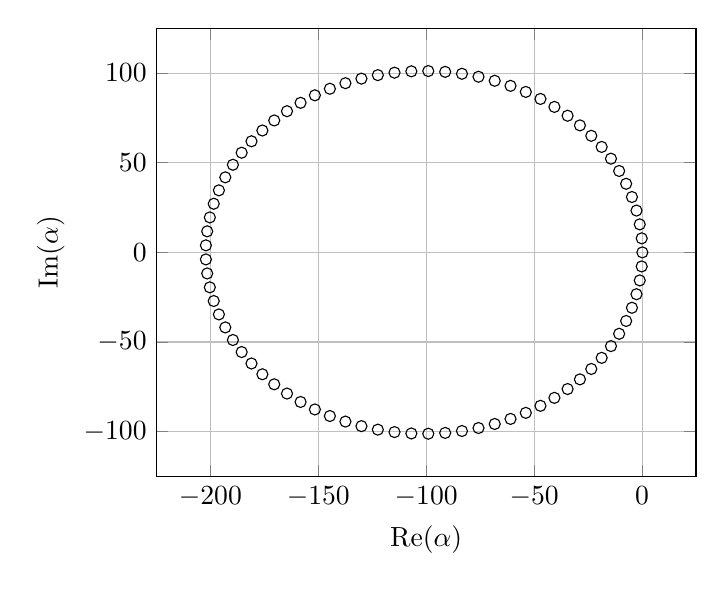
\begin{tikzpicture}
	\begin{axis}[xmin=-225, xmax=25, 
                   ymin=-125, ymax=125, 
                   %extra x ticks={-150,-50,0}, 
                   %extra y ticks={-100,-50,0,50}, 
                   %extra tick style={grid=major}, ]
                   xlabel = {Re($\alpha$)},
                   ylabel = {Im($\alpha$)},
                   tick style={grid=major},
                   ]
		                   
	\addplot [only marks, mark=o] coordinates { 
		(-202.061585, 3.921650) 
(-202.061585, -3.921650) 
(-201.453789, 11.741364) 
(-201.453789, -11.741364) 
(-200.241852, 19.490464) 
(-200.241852, -19.490464) 
(-198.433063, 27.122347) 
(-198.433063, -27.122347) 
(-196.038299, 34.591112) 
(-196.038299, -34.591112) 
(-193.071965, 41.851842) 
(-193.071965, -41.851842) 
(-189.551898, 48.860871) 
(-189.551898, -48.860871) 
(-185.499270, 55.576044) 
(-185.499270, -55.576044) 
(-180.938454, 61.956977) 
(-180.938454, -61.956977) 
(-175.896878, 67.965293) 
(-175.896878, -67.965293) 
(-170.404864, 73.564858) 
(-170.404864, -73.564858) 
(-164.495440, 78.721995) 
(-164.495440, -78.721995) 
(-158.204148, 83.405688) 
(-158.204148, -83.405688) 
(-151.568823, 87.587770) 
(-151.568823, -87.587770) 
(-144.629371, 91.243089) 
(-144.629371, -91.243089) 
(-137.427527, 94.349662) 
(-137.427527, -94.349662) 
(-130.006604, 96.888804) 
(-130.006604, -96.888804) 
(-122.411231, 98.845245) 
(-122.411231, -98.845245) 
(-114.687089, 100.207220) 
(-114.687089, -100.207220) 
(-106.880631, 100.966537) 
(-106.880631, -100.966537) 
(-99.038806, 101.118629) 
(-99.038806, -101.118629) 
(-91.208776, 100.662581) 
(-91.208776, -100.662581) 
(-83.437632, 99.601138) 
(-83.437632, -99.601138) 
(-75.772110, 97.940681) 
(-75.772110, -97.940681) 
(-68.258311, 95.691197) 
(-68.258311, -95.691197) 
(-60.941425, 92.866215) 
(-60.941425, -92.866215) 
(-53.865456, 89.482725) 
(-53.865456, -89.482725) 
(-47.072959, 85.561075) 
(-47.072959, -85.561075) 
(-40.604786, 81.124851) 
(-40.604786, -81.124851) 
(-34.499837, 76.200733) 
(-34.499837, -76.200733) 
(-28.794827, 70.818334) 
(-28.794827, -70.818334) 
(-23.524069, 65.010025) 
(-23.524069, -65.010025) 
(-18.719259, 58.810739) 
(-18.719259, -58.810739) 
(-14.409295, 52.257758) 
(-14.409295, -52.257758) 
(0.137646, 0.000000) 
(-0.166481, 7.837401) 
(-0.166481, -7.837401) 
(-1.077033, 15.627667) 
(-1.077033, -15.627667) 
(-2.588533, 23.323946) 
(-2.588533, -23.323946) 
(-4.691891, 30.879953) 
(-4.691891, -30.879953) 
(-10.620099, 45.390492) 
(-10.620099, -45.390492) 
(-7.374457, 38.250243) 
(-7.374457, -38.250243) 

		};                   
	\end{axis}
\end{tikzpicture}}
\caption{Alpha-Eigenvalue Spectrum for Problem 5.2.2.1}
\label{fig:G81Spec}
\end{figure}

\clearpage

\begin{table}[!htbp]
	\caption{Transport Sweep Comparisons for Problem 5.2.2.1}
	\label{table:G81a}
	\begin{subtable}[h]{1.0\textwidth}
	\centering\ra{1.3}
	\begin{tabular}{@{}ccc@{}}\toprule
	& \multicolumn{2}{c}{Transport Sweeps} \\
	\cmidrule{2-3} $\alpha$  (s$^{-1}) $& RQFP & Critical Search \\
	\midrule
	0.13765 & * & 63,843 \\
	\bottomrule
	\multicolumn{3}{l}{*Did Not Converge}
	\end{tabular}
	\caption{Alpha-Eigenvalue: Comparison of RQFP and Critical Search Sweeps}
	\label{table:AlphaProb5221}
	\end{subtable}%
	\vspace{0.25cm}
	\begin{subtable}[h]{1.0\textwidth}
	\centering\ra{1.3}
	\begin{tabular}{@{}ccc@{}}\toprule
	& \multicolumn{2}{c}{Transport Sweeps} \\
	\cmidrule{2-3} $k_{\text{eff}}$ & RQFP & Power Method \\
	\midrule
	1.11663 & 6,701 & 6,707 \\
	\bottomrule
	\end{tabular}
	\caption{$k$-Effective: Comparison of RQFP and Critical Search Sweeps}
	\label{table:kProb5221}
	\end{subtable}%
\end{table}

\textbf{Problem 5.2.2.2}: We consider a problem similar to Problem 5.2.1.1 where the energy group velocities are group-dependent. The velocity of each group is given by $v_{g} = 82 - g$ and the cross sections are the same as Problem 5.2.1.1 (Table~\ref{table:G81v}). The $k$-effective eigenvalue remains 1.11663 as only the velocity terms have been modified. The problem no longer has an analytical expression for the alpha-eigenvalue spectrum. The dominant alpha-eigenvalue is found to be $2.2464$ s$^{-1}$ from numerical eigenvalue solvers. With the change in the velocity, the alpha-eigenvalue spectrum eigenvalues are no longer on a circle (Figure~\ref{fig:G81VSpec}). Instead, the eigenvalues are along elliptical shapes with very negative real eigenvalues now existing. 

%We also note that there are complex eigenvalues whose real parts are larger than zero, a phenomenon unexpected for alpha-eigenvalue problems where only the dominant eigenvalue has real part larger than zero for supercritical systems.

Similar to Problem 5.2.2.1, the alpha-eigenvalue Rayleigh Quotient Fixed Point method does not converge for this method. The spectral radius of the Jacobian matrix for the fixed-point formulation evaluated at the fixed point is found to be larger than one, implying the method will not converge for this problem. The critical search method is able to converge the alpha-eigenvalue. However, it requires a large number of iterations (Table~\ref{table:AlphaProb5222}).

Also similar to Problem 5.2.2.1, both the Rayleigh Quotient Fixed Point method and power method were able to converge the $k$-effective eigenvalue. This is expected as the only change from Problem 5.2.2.1 was in the group velocities which do not matter in the $k$-effective eigenvalue problem. The number of transport sweeps required to converge the problem did not change (Table~\ref{table:kProb5222}).

\begin{table}[!htbp]
    \centering
    \caption{Infinite-Medium 81-Group Problem Cross Sections (cm$^{-1}$), Velocity Modification}
\label{table:G81v}
    \begin{tabular}{*7c}
        \toprule
	$g$ & $\sigma$ & $\sigma_{f}$ & $\sigma_{sg,g+1}$ & $\chi$ & $v_{g}$ [cm/s] \\ 
        \midrule
	1 & 101.0 & 0.0 & 100.0 & 1.0 & 1.0 \\
	2-80 & 101.0 & 0.0 & 100.0 & 0.0 & 2.0-80.0 \\
	81 & 101.0 & 100.0 & 0.0 & 0.0 & 81.0 \\
        \bottomrule
    \end{tabular}
\end{table}

\begin{figure}[!htbp]
\centering
	\resizebox{0.90\textwidth}{!}{
	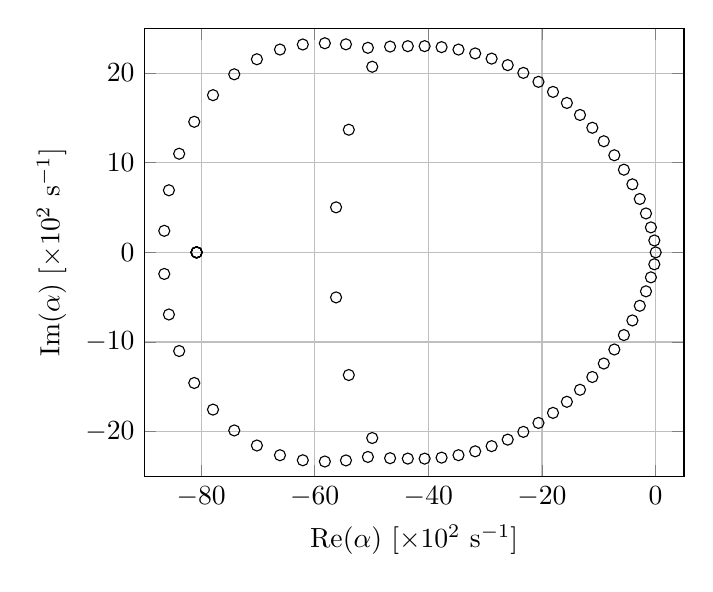
\begin{tikzpicture}
	\begin{axis}[xmin=-90, xmax=5, 
                   ymin=-25, ymax=25, 
                   %extra x ticks={-150,-50,0}, 
                   %extra y ticks={-100,-50,0,50}, 
                   %extra tick style={grid=major}, ]
                   xlabel = {Re($\alpha$) [$\times 10^{2}$ s$^{-1}$]},
                   ylabel = {Im($\alpha$) [$\times 10^{2}$ s$^{-1}$]},
                   tick style={grid=major},
                   ]

	\addplot [only marks, mark=o] coordinates { 
	(0.022464, 0.000000) 
(-0.218203, 1.326098) 
(-0.218203, -1.326098) 
(-0.821089, 2.786275) 
(-0.821089, -2.786275) 
(-1.685632, 4.343614) 
(-1.685632, -4.343614) 
(-2.777473, 5.955446) 
(-2.777473, -5.955446) 
(-4.078351, 7.590189) 
(-4.078351, -7.590189) 
(-5.575099, 9.222346) 
(-5.575099, -9.222346) 
(-7.256446, 10.830170) 
(-7.256446, -10.830170) 
(-9.111739, 12.394535) 
(-9.111739, -12.394535) 
(-11.130351, 13.898327) 
(-11.130351, -13.898327) 
(-13.301379, 15.326118) 
(-13.301379, -15.326118) 
(-15.613491, 16.663970) 
(-15.613491, -16.663970) 
(-18.054858, 17.899323) 
(-18.054858, -17.899323) 
(-20.613133, 19.020937) 
(-20.613133, -19.020937) 
(-23.275457, 20.018860) 
(-23.275457, -20.018860) 
(-26.028493, 20.884415) 
(-26.028493, -20.884415) 
(-28.858471, 21.610190) 
(-28.858471, -21.610190) 
(-31.751212, 22.190078) 
(-31.751212, -22.190078) 
(-34.692549, 22.619413) 
(-34.692549, -22.619413) 
(-37.668777, 22.892639) 
(-37.668777, -22.892639) 
(-40.654267, 23.002823) 
(-40.654267, -23.002823) 
(-43.616536, 22.999684) 
(-43.616536, -22.999684) 
(-46.734165, 22.954101) 
(-46.734165, -22.954101) 
(-50.642538, 22.814456) 
(-50.642538, -22.814456) 
(-49.876538, 20.703484) 
(-49.876538, -20.703484) 
(-56.241271, 5.022065) 
(-56.241271, -5.022065) 
(-54.002418, 13.679548) 
(-54.002418, -13.679548) 
(-54.504562, 23.203205) 
(-54.504562, -23.203205) 
(-58.222639, 23.324428) 
(-58.222639, -23.324428) 
(-62.098762, 23.185273) 
(-62.098762, -23.185273) 
(-66.119818, 22.622868) 
(-66.119818, -22.622868) 
(-70.181511, 21.539475) 
(-70.181511, -21.539475) 
(-74.165691, 19.860233) 
(-74.165691, -19.860233) 
(-77.907161, 17.534907) 
(-77.907161, -17.534907) 
(-81.209788, 14.565329) 
(-81.209788, -14.565329) 
(-83.866013, 11.001706) 
(-83.866013, -11.001706) 
(-85.671259, 6.927196) 
(-85.671259, -6.927196) 
(-86.489088, 2.404467) 
(-86.489088, -2.404467) 
(-80.800000, 0.000000) 
(-80.800000, 0.000000) 
(-80.800000, 0.000000) 
(-80.800000, 0.000000) 
(-80.800000, 0.000000) 
(-80.800000, 0.000000) 

	};
\end{axis}
\end{tikzpicture}}
\caption{Alpha-Eigenvalue Spectrum for Problem 5.2.2.2}
\label{fig:G81VSpec}
\end{figure}

%\begin{table}[!htbp]
%    \centering
%    \caption{Transport Sweeps for Convergence for Problem 5.2.2.2}
%\label{table:G81b}
%    \scalebox{1.00}{
%    \begin{tabular}{*4c}
%        \toprule
%        \multicolumn{4}{c}{Transport Sweeps} \\
%        \cmidrule(lr){1-4}
%        $k$RQ & $k$PM & $\alpha$RQ & $\alpha$CS \\
%        \midrule
%	6701 & 6707 & * & 50773 \\
%        \bottomrule
%        \multicolumn{2}{c}{*Did Not Converge}
%    \end{tabular}
%    }
%\end{table}

\clearpage

\begin{table}[!htbp]
	\caption{Transport Sweep Comparisons for Problem 5.2.2.2}
	\begin{subtable}[h]{1.0\textwidth}
	\centering\ra{1.3}
	\begin{tabular}{@{}ccc@{}}\toprule
	& \multicolumn{2}{c}{Transport Sweeps} \\
	\cmidrule{2-3} $\alpha$  (s$^{-1}) $& RQFP & Critical Search \\
	\midrule
	2.2464 & * & 50,773 \\
	\bottomrule
	\multicolumn{3}{l}{*Did Not Converge}
	\end{tabular}
	\caption{Alpha-Eigenvalue: Comparison of RQFP and Critical Search Sweeps}
	\label{table:AlphaProb5222}
	\end{subtable}%
	\vspace{0.25cm}
	\begin{subtable}[h]{1.0\textwidth}
	\centering\ra{1.3}
	\begin{tabular}{@{}ccc@{}}\toprule
	& \multicolumn{2}{c}{Transport Sweeps} \\
	\cmidrule{2-3} $k_{\text{eff}}$ & RQFP & Power Method \\
	\midrule
	1.11663 & 6,701 & 6,707 \\
	\bottomrule
	\end{tabular}
	\caption{$k$-Effective: Comparison of RQFP and Critical Search Sweeps}
	\label{table:kProb5222}
	\end{subtable}%
\end{table}

\textbf{Problem 5.2.2.3}: We consider another problem similar to Problem 5.2.1.1 where we now allow downscattering from energy group $g \rightarrow g'$ over several energy groups with equal probability where $g + 1 \leq g' \leq g+5$. For the last five energy groups, the downscattering cross section is equally distributed among the remaining groups where $g+1 \leq g' \leq G$. The total scattering cross section remains unchanged. The $k$-effective eigenvalue is 1.8853 and the alpha-eigenvalue is $2.2914$ s$^{-1}$.

The alpha-eigenvalue spectrum seen in Figure~\ref{fig:G81P3Spec} is significantly different to that of Problem 5.2.2.1. The spectrum contains more eigenvalues with large real negative parts. This is due to neutrons being able to downscatter quickly by skipping several energy groups.

The alpha-eigenvalue Rayleigh Quotient Fixed Point method was able to converge on the analytical alpha-eigenvalue. By allowing downscattering to more energy groups, the Jacobian of the fixed-point method at the fixed point is now less than one, allowing the convergence of the method (Section~\ref{sec:JacobAlpha}). In this particular problem, the alpha-eigenvalue RQFP method vastly outperforms the critical search method. The critical search method requires 20 times the number of sweeps the RQFP method does (Table~\ref{table:AlphaProb5223}). This is caused by the need for multiple $k$-effective eigenvalue calculations to bracket the alpha-eigenvalue.

Both the Rayleigh Quotient Fixed Point method and power method with fission norm update were able to converge the eigenvalue and eigenvector for the $k$-effective eigenvalue problem requiring a similar number of iterations (Table~\ref{table:kProb5223}). 

\begin{figure}[!htbp]
\centering
	\resizebox{0.90\textwidth}{!}{
	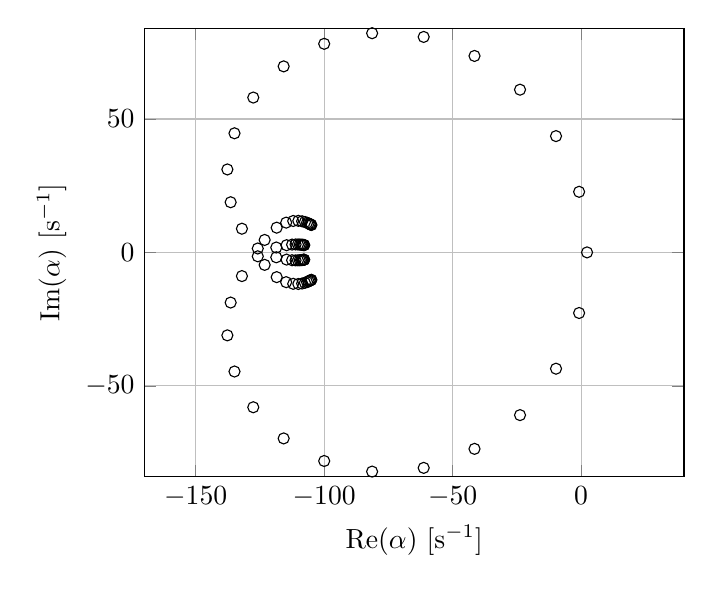
\begin{tikzpicture}
	\begin{axis}[xmin=-170, xmax=40, 
                   ymin=-84, ymax=84, 
                   %extra x ticks={-150,-50,0}, 
                   %extra y ticks={-100,-50,0,50}, 
                   %extra tick style={grid=major}, ]
                   xlabel = {Re($\alpha$) [s$^{-1}$]},
                   ylabel = {Im($\alpha$) [s$^{-1}$]},
                   tick style={grid=major},
                   ]

	\addplot [only marks, mark=o] coordinates {
	(2.291412, 0.000000) 
(-0.801864, 22.705383) 
(-0.801864, -22.705383) 
(-9.783631, 43.575028) 
(-9.783631, -43.575028) 
(-23.793621, 60.968847) 
(-23.793621, -60.968847) 
(-41.507004, 73.614858) 
(-41.507004, -73.614858) 
(-61.283845, 80.738172) 
(-61.283845, -80.738172) 
(-81.352261, 82.131623) 
(-81.352261, -82.131623) 
(-100.003253, 78.160415) 
(-100.003253, -78.160415) 
(-115.774060, 69.701268) 
(-115.774060, -69.701268) 
(-127.598815, 58.024469) 
(-127.598815, -58.024469) 
(-134.909876, 44.633856) 
(-134.909876, -44.633856) 
(-137.680045, 31.084029) 
(-137.680045, -31.084029) 
(-136.403691, 18.795038) 
(-136.403691, -18.795038) 
(-132.020625, 8.876563) 
(-132.020625, -8.876563) 
(-125.852372, 1.461794) 
(-125.852372, -1.461794) 
(-123.173721, 4.669417) 
(-123.173721, -4.669417) 
(-118.491174, 9.268922) 
(-118.491174, -9.268922) 
(-114.800269, 11.150988) 
(-114.800269, -11.150988) 
(-118.641632, 1.835834) 
(-118.641632, -1.835834) 
(-112.063558, 11.769920) 
(-112.063558, -11.769920) 
(-110.061707, 11.831358) 
(-110.061707, -11.831358) 
(-108.590864, 11.656313) 
(-108.590864, -11.656313) 
(-107.501612, 11.395004) 
(-107.501612, -11.395004) 
(-114.640317, 2.695387) 
(-114.640317, -2.695387) 
(-106.690513, 11.119391) 
(-106.690513, -11.119391) 
(-106.086882, 10.864281) 
(-106.086882, -10.864281) 
(-105.642490, 10.646364) 
(-105.642490, -10.646364) 
(-105.324539, 10.473385) 
(-105.324539, -10.473385) 
(-105.111091, 10.348707) 
(-105.111091, -10.348707) 
(-104.988176, 10.273633) 
(-104.988176, -10.273633) 
(-112.492061, 2.931144) 
(-112.492061, -2.931144) 
(-111.140110, 2.982538) 
(-111.140110, -2.982538) 
(-110.210112, 2.970403) 
(-110.210112, -2.970403) 
(-109.534381, 2.935693) 
(-109.534381, -2.935693) 
(-109.027033, 2.894605) 
(-109.027033, -2.894605) 
(-108.639617, 2.854226) 
(-108.639617, -2.854226) 
(-108.342829, 2.817867) 
(-108.342829, -2.817867) 
(-108.118070, 2.787129) 
(-108.118070, -2.787129) 
(-107.774437, 2.734682) 
(-107.774437, -2.734682) 
(-107.953214, 2.762799) 
(-107.953214, -2.762799) 
(-107.840334, 2.745257) 
(-107.840334, -2.745257) 

		};
\end{axis}
\end{tikzpicture}}
\caption{Alpha-Eigenvalue Spectrum for Problem 5.2.2.3}
\label{fig:G81P3Spec}
\end{figure}

%\begin{table}[!htbp]
%    \centering
%    \caption{Transport Sweeps for Convergence for Problem 5.2.2.3}
%\label{table:G81c}
%    \scalebox{1.00}{
%    \begin{tabular}{*4c}
%        \toprule
%        \multicolumn{4}{c}{Transport Sweeps} \\
%        \cmidrule(lr){1-4}
%        $k$RQ & $k$PM & $\alpha$RQ & $\alpha$CS \\
%        \midrule
%	5306 & 5080 & 5516 & 105570 \\
%        \bottomrule
%        \multicolumn{2}{c}{*Did Not Converge}
%    \end{tabular}
%    }
%\end{table}

\begin{table}[!htbp]
	\caption{Transport Sweep Comparisons for Problem 5.2.2.3}
	\begin{subtable}[h]{1.0\textwidth}
	\centering\ra{1.3}
	\begin{tabular}{@{}ccc@{}}\toprule
	& \multicolumn{2}{c}{Transport Sweeps} \\
	\cmidrule{2-3} $\alpha$  (s$^{-1}) $& RQFP & Critical Search \\
	\midrule
	2.2914 & 5,516 & 105,570 \\
	\bottomrule
	\end{tabular}
	\caption{Alpha-Eigenvalue: Comparison of RQFP and Critical Search Sweeps}
	\label{table:AlphaProb5223}
	\end{subtable}%
	\vspace{0.25cm}
	\begin{subtable}[h]{1.0\textwidth}
	\centering\ra{1.3}
	\begin{tabular}{@{}ccc@{}}\toprule
	& \multicolumn{2}{c}{Transport Sweeps} \\
	\cmidrule{2-3} $k_{\text{eff}}$ & RQFP & Power Method \\
	\midrule
	1.8853 & 5,306 & 5,080 \\
	\bottomrule
	\end{tabular}
	\caption{$k$-Effective: Comparison of RQFP and Critical Search Sweeps}
	\label{table:kProb5223}
	\end{subtable}%
\end{table}


\label{sec:Res}

\section{Conclusion}

The RQFP method for alpha- and $k$-effective eigenvalues performs well for infinite-medium problems, reducing in certain cases the number of iterations up to a factor of twenty. For the alpha-eigenvalue RQFP method, the method is able to converge subcritical systems without issue. For a certain class of problems with unphysical cross sections, the alpha-eigenvalue RQFP method fails to converge. This failure to converge is caused by the structure of the alpha-eigenvalue spectrum. However, these problems are special cases, with unphysical data such as unit velocity in all energy groups. For these particular problems, it is found that the spectral radius of the Jacobian matrix implies convergence is not possible. For this reason, we believe the alpha-eigenvalue RQFP method is robust for all infinite-medium problems of interest. The RQFP method for $k$-effective eigenvalue calculations performed better or similar to the power method with a fission norm update for the eigenvalue. For problems where only the number of neutrons emitted in fission was varied, the RQFP method took a similar number of iterations to converge for all problems, no matter the criticality of the system. This suggests that the method's convergence is determined by the eigenvector shape rather than the eigenvalue.

%\begin{table}[H]
%    \centering
%    \caption{\textbf{Criticality Benchmark Problem List and Properties} \cite{sood2003analytical}}
%\label{table:probs}
%    %\rowcolors{5}{}{gray!10}
%    \scalebox{1.00}{
%    %\scalebox{0.95}{
%    \begin{tabular}{*7c}
%        \toprule
%        & \multicolumn{6}{c}{Problem Properties} \\
%        \cmidrule(lr){2-7}
%        Problem & 1D  & 1D & Infinite & Reflected & Reference & Reference \\    
%        ID   & Slab & Spherical     & Medium & BC & $k_{\text{eff}}$  & $\alpha$ \\
%        \midrule
%        PUa-1-0-IN &        &  & \CHECK   & &  2.612903    \\
%        PUa-1-0-SL & \CHECK        &        &  &  &  1.00 \\
%        PUb-1-0-IN &        &  & \CHECK  & & 2.290323 \\
%        PUa-H2O(1)-1-0-SL & \CHECK &  &   & \CHECK & 1.00     \\
%        PUa-H2O(0.5)-1-0-SL & \CHECK & & & \CHECK & 1.00    \\
%        PUb-1-0-SL & \CHECK &        & &  & 1.00 \\
%        PUb-1-0-SP &  & \CHECK & &  & 1.00 \\
%        Ua-1-0-SL & \CHECK & & & & 1.00 \\
%	Ua-1-0-IN & & & \CHECK & & 2.25 \\
%	Ub-1-0-IN & & & \CHECK & & 2.330917 \\
%	Uc-1-0-IN & & & \CHECK & & 2.256083 \\
%	Ud-1-0-IN & & & \CHECK & & 2.232667 \\
%        \bottomrule
%    \end{tabular}
%    }
%\end{table}